\documentclass[10pt]{article}

\usepackage[utf8]{inputenc}
\usepackage[T1]{fontenc}
\usepackage[english]{babel}
\usepackage[a4paper, bmargin=30mm, tmargin=30mm]{geometry}

\usepackage{graphicx,calc}
\graphicspath{ {img/} }

\usepackage{amsmath, amssymb, amsfonts}

\usepackage{relsize}
\usepackage{xcolor}
\usepackage{parskip}
\usepackage{caption}
\usepackage{subcaption}
\usepackage{booktabs}
\usepackage{colortbl}
\usepackage{array}
\usepackage{listings}
\usepackage{hyperref}
\hypersetup{
	colorlinks = true,
	urlcolor = {blue},
}

\definecolor{codegreen}{rgb}{0,0.6,0}
\definecolor{codegray}{rgb}{0.5,0.5,0.5}
\definecolor{codepurple}{rgb}{0.58,0,0.82}
\definecolor{backcolor}{rgb}{0.90,0.90,0.87}

\lstdefinestyle{cmdStyle}{
	backgroundcolor=\color{backcolor},
	basicstyle=\ttfamily\footnotesize,
	breakatwhitespace=false,
	breaklines=true,
	captionpos=b,
	keepspaces=true,
	showspaces=false,
	showtabs=false,
	tabsize=4
}
\lstset{style=cmdStyle}

\colorlet{tabrowcolorA}{gray!10}
\newcommand{\tabrowA}{\rowcolor{tabrowcolorA}}

%\renewcommand{\_}{\textscale{0.5}{\textunderscore}}

\begin{document}

\begin{center}
{\huge Customized Plastic Extruder}\\
\vspace{0.2cm}
{\large For mounting on franka emika panda and use with ROS2-Control}\\
\vspace{0.4cm}
\hrule
\vspace{0.0cm}
{%
\setlength\tabcolsep{6pt} %default value: 6pt
\begin{tabular}{ll}
	Author/Creator: & Andreas Moltumyr \\
	E-mail: & andreas.h.moltumyr@gmail.com \\
	Last modified: & \today
\end{tabular}
}%
\vspace{0.2cm}
\hrule
\vspace{1.5cm}
\end{center}

\section{Intro}
The purpose of this document is to give useful information about the extruder in the picture and explain how to use it with ROS2. It is meant to be mounted to the fingers of a franka emika panda robot.  Links to hardware, software and CAD resources can be found below. Usage is described below.


\begin{figure}[h]
\centering
\begin{minipage}{0.48\textwidth}
	\centering
	{%
	\setlength{\fboxsep}{0pt}%
	\setlength{\fboxrule}{1pt}%
	\fbox{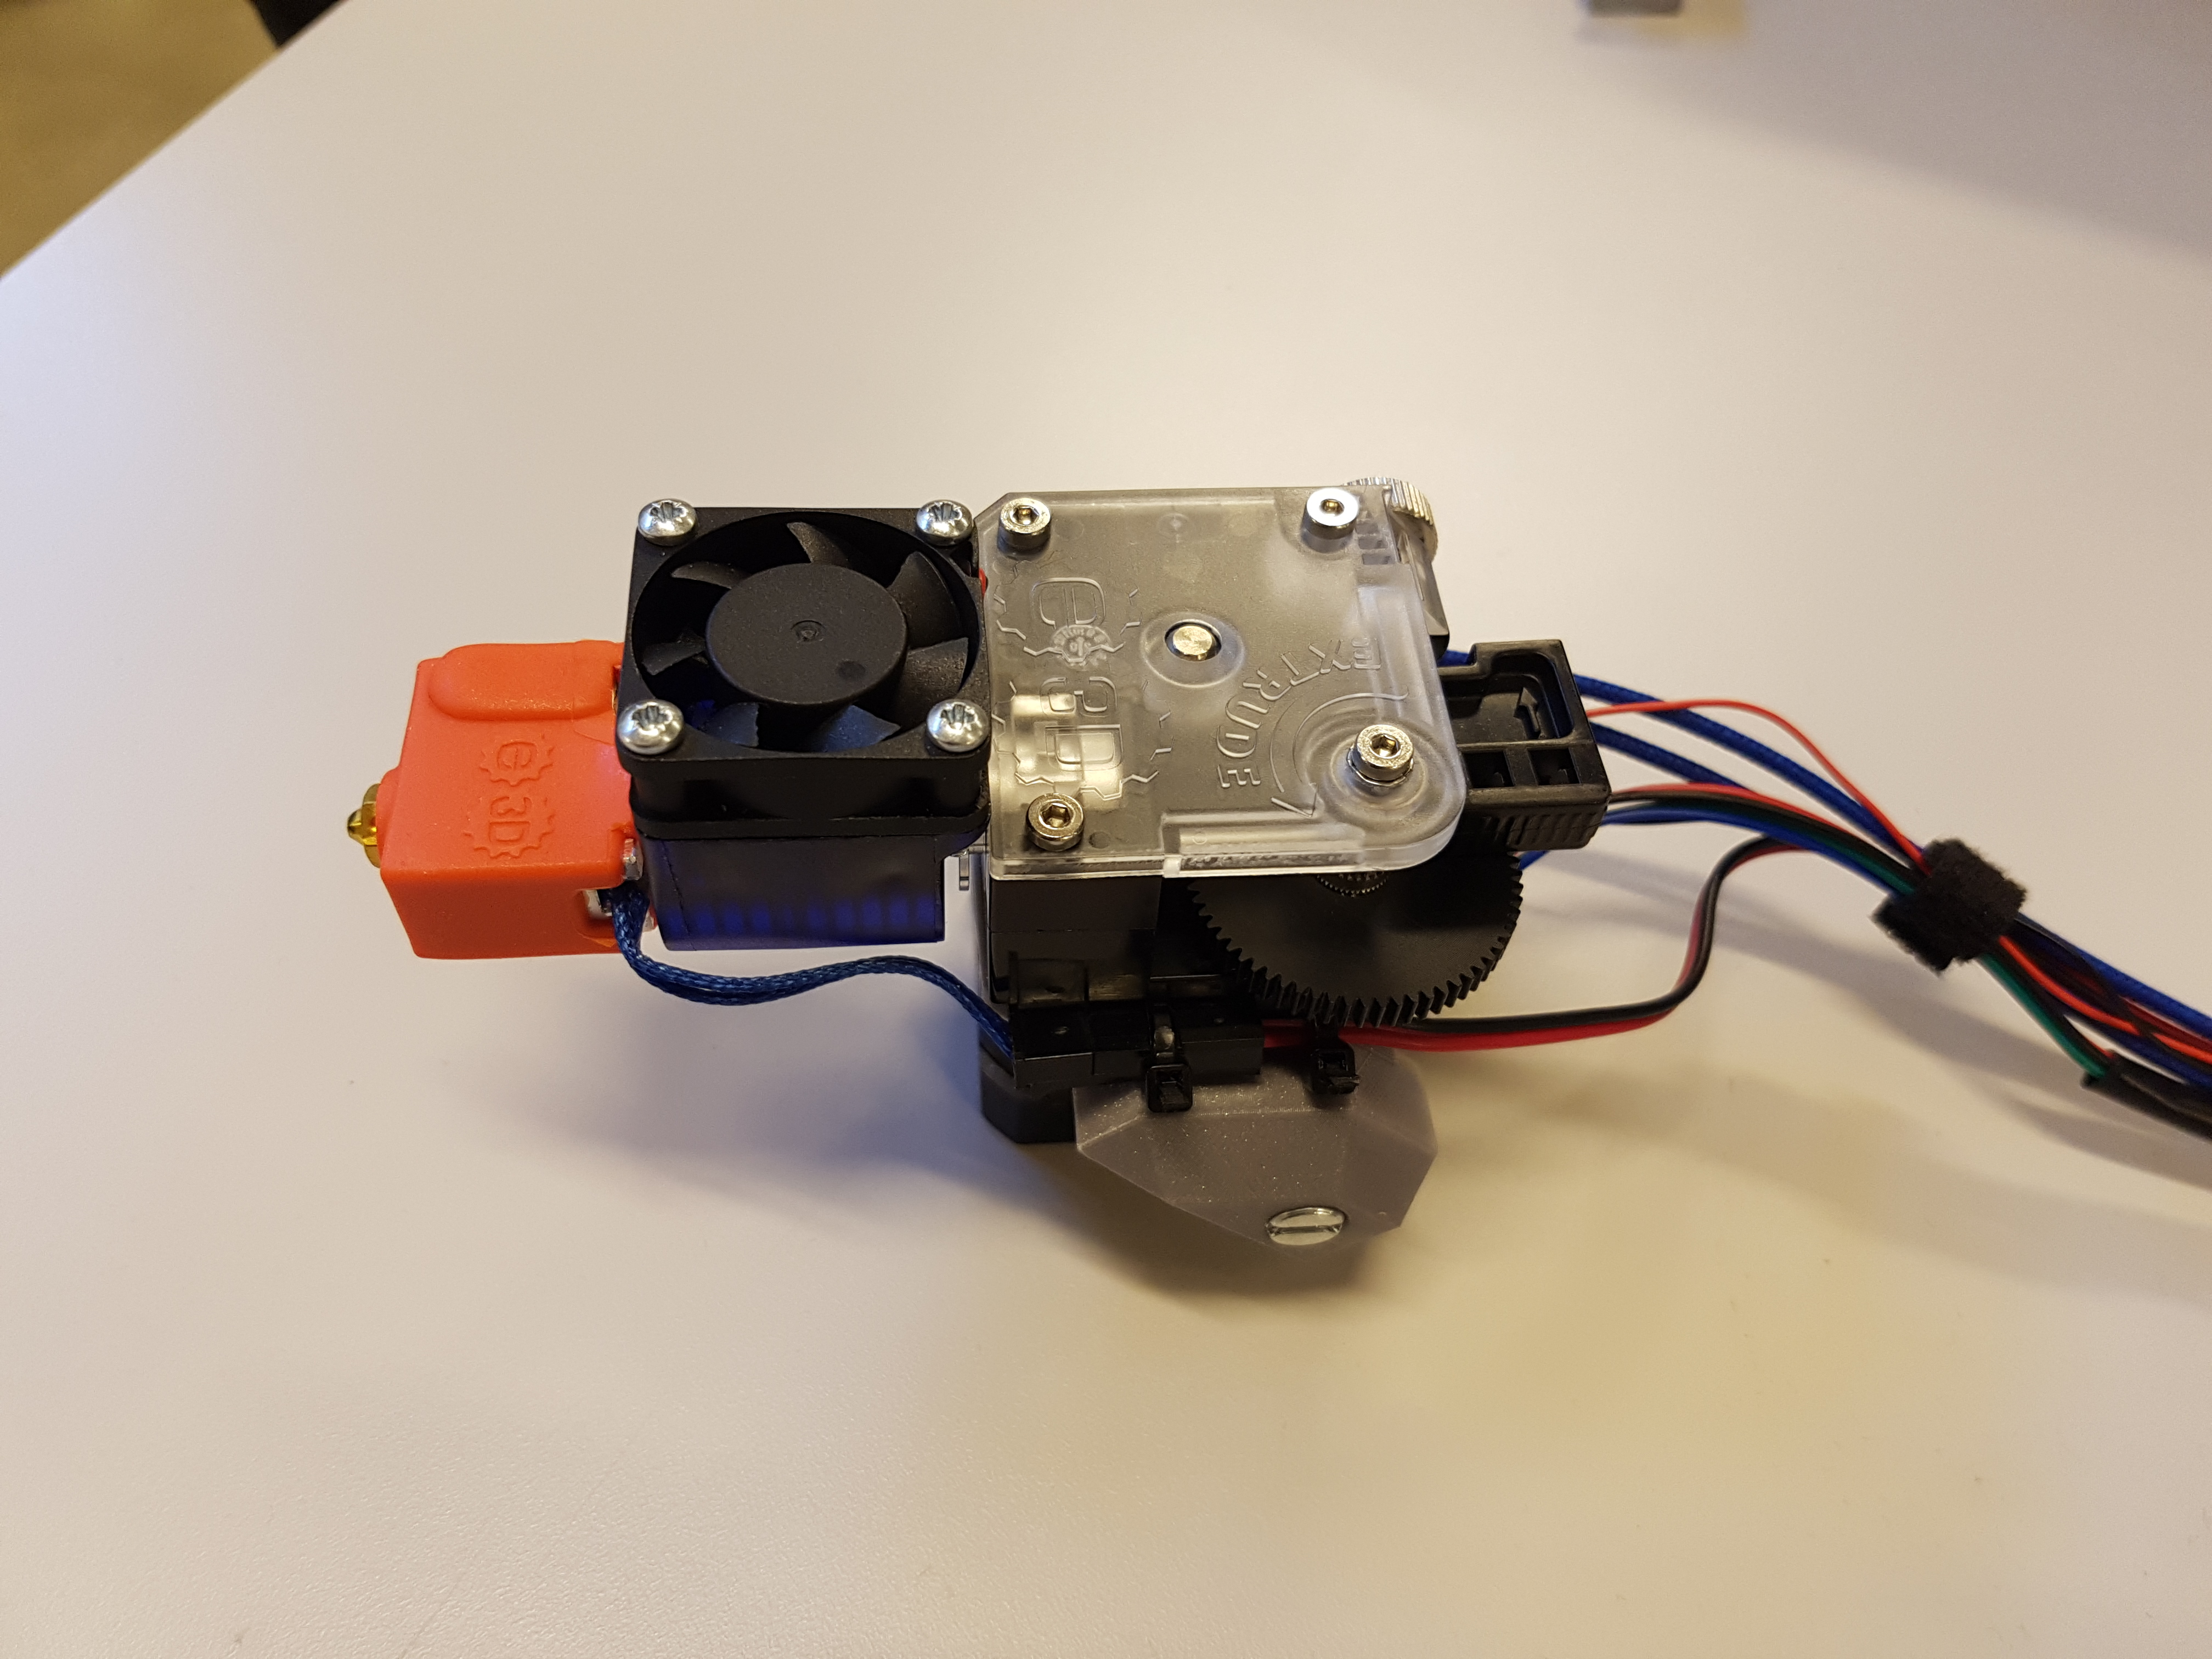
\includegraphics[trim={13cm 7cm 0 14cm}, clip, width=\linewidth]{extruder.jpg}}%
	}%
	\caption{Extruder}
\end{minipage}\hfill
\begin{minipage}{0.48\textwidth}
	\centering
	{%
	\setlength{\fboxsep}{0pt}%
	\setlength{\fboxrule}{1pt}%
	\fbox{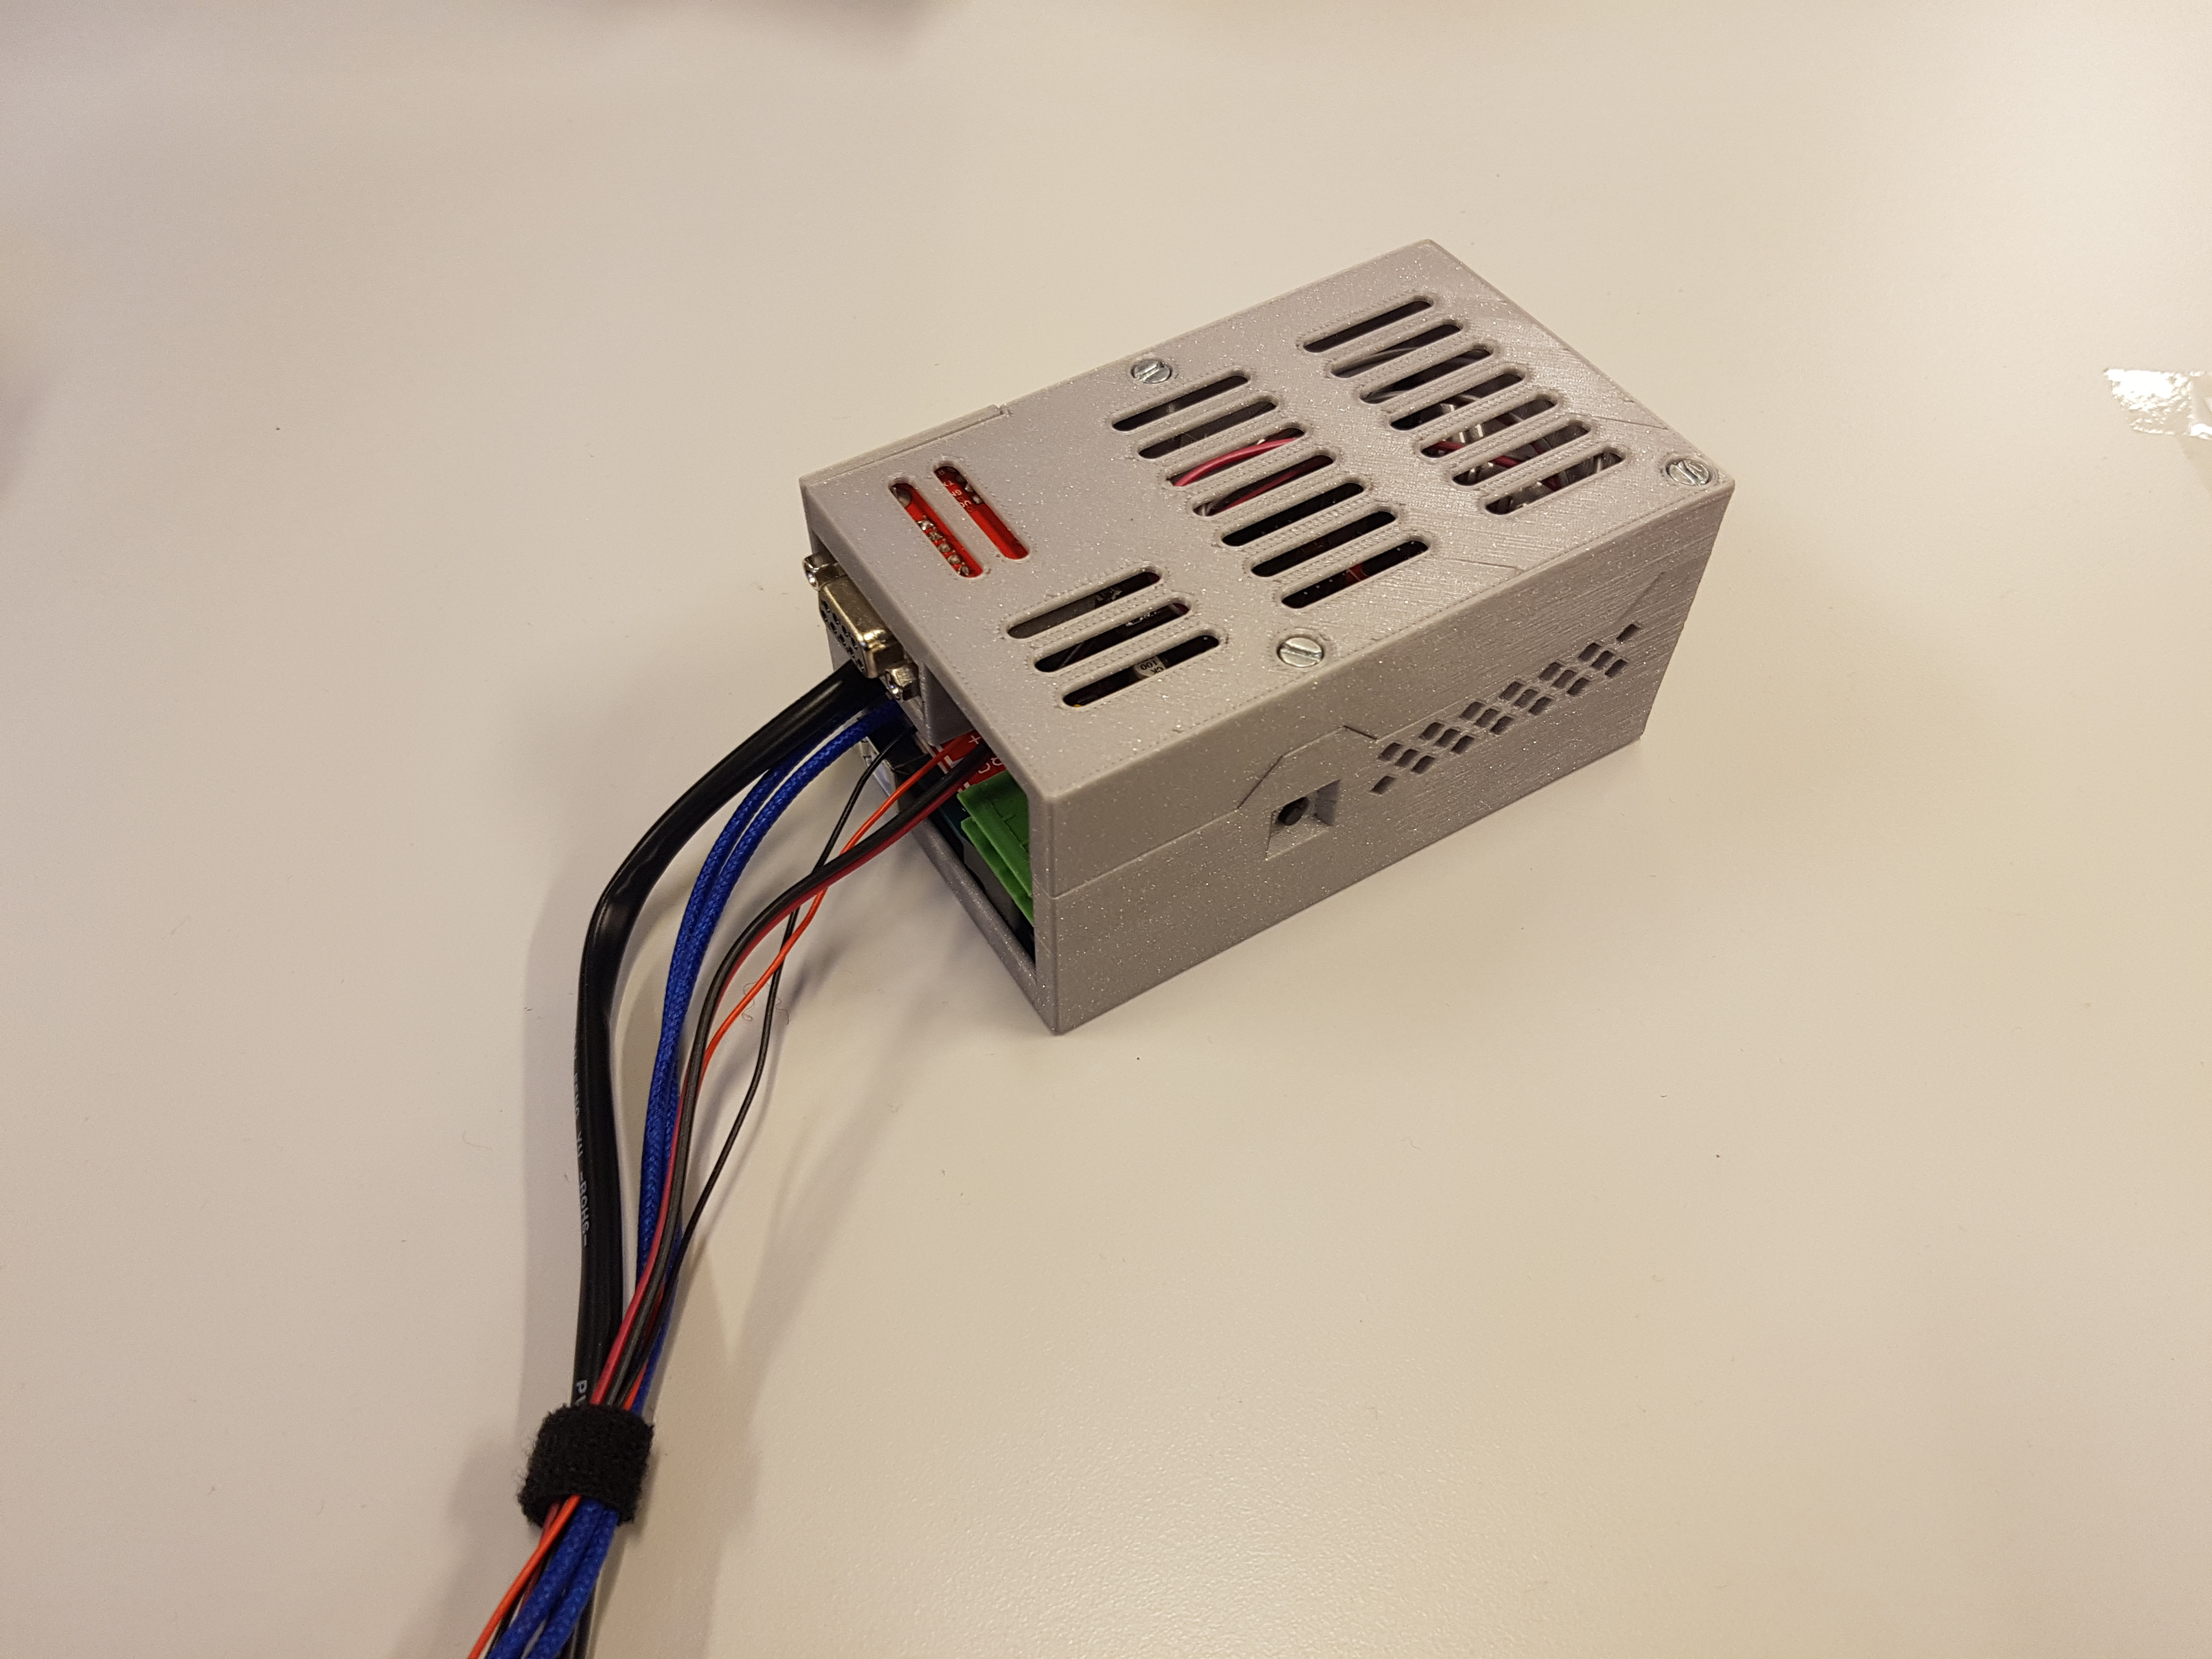
\includegraphics[trim={6cm 17cm 7cm 4cm}, clip, width=\linewidth]{control_box.jpg}}%
	}%
	\caption{Control box}
\end{minipage}
\end{figure}


\begin{table}[h]
	\centering
	{
	\captionsetup{width=\linewidth}
	\caption{Miscellaneous extruder data}
	}
	\vspace{-0.6em}
	\setlength\tabcolsep{6pt} %default value: 6pt
	\begin{tabular}{lc}
	\toprule
	Parameter & Value \\
	\midrule
	Filament diameter & $2.85$ mm  \\
	Nozzle diameter & $0.8$ mm \\
	Stepper motor steps per revolution & $400$ \\
	Heater cartridge power rating & $30$ Watts \\
	Input voltage to extruder (ramp/arduino control box) & $12$ Volts \\
	Current draw at 12 Volts & $0.5 \sim 3$ Amperes \\
	Current draw (only stepper) & $\sim 0.5$ Amperes \\
	Current draw (only heater)  & $0 \sim 2.5$ Amperes \\
	\bottomrule
	\end{tabular}
\end{table}

\newpage
\section{Resources}
\begin{table}[h]
	\centering
	{
	\captionsetup{width=\linewidth}
	\caption{Part list}
	\label{}
	}
	\vspace{-0.6em}
	\setlength\tabcolsep{6pt} %default value: 6pt
	\begin{tabular}{p{0.35\linewidth}p{0.65\linewidth}}
	\toprule
	Parts & Notes \\
	\midrule
	\tabrowA \href{https://e3d-online.com/products/titan-extruder}{Titan extruder} & 2.85mm filament diameter, direct drive, with `\href{https://e3d-online.com/products/motors}{compact but powerful motor}' (\href{https://e3d-online.zendesk.com/hc/en-us/article_attachments/360016616377/Compact_But_Powerful_Motor.pdf}{datasheet}). \\
	\href{https://e3d-online.com/products/volcano-hotend}{Volcano HotEnd} & 2.85mm filament diameter, direct drive, 12V. with 0.8mm brass nozzle.  \\
	\tabrowA \href{https://store.arduino.cc/products/arduino-mega-2560-rev3}{Arduino Mega 2560 Rev3} & \href{https://docs.arduino.cc/hardware/mega-2560}{Docs/Resources}, \href{https://www.arduino.cc/reference/en/}{arduino C++ reference} \\
	\href{https://www.electrokit.com/produkt/ramps-1-4-shield}{Ramps 1.4} & \href{https://reprap.org/wiki/RAMPS_1.4}{Docs}. Supports control of five stepper motors, fans, nozzle heating and bed heating. However, the extruder are only using one motor, nozzle heating and a fan. \\
	\tabrowA \href{https://www.electrokit.com/produkt/stegmotordrivare-drv8825/}{DRV8825, Stepper motor driver} & \href{https://www.electrokit.com/uploads/productfile/41016/drv8825.pdf}{Datasheet}. \\
	\href{https://www.sparkfun.com/products/449}{RS-232 til TTL nivåomformer} & \href{https://github.com/sparkfun/RS232_Shifter_SMD}{Docs}. \\
	\tabrowA \href{http://www.sunrichtech.com.hk/ProductShow.aspx?Mid=1&pid=419}{PCIe RS232 computer card} &  \\
	RS232 cable &  \\
	\tabrowA \href{https://www.e3printable.no/nettbutikk-norge/83-byggeplate/345-pei-byggeplate/?variantId=215}{PEI sheet} & To print on top of. Should improve adhesion of first layer. \\
	PLA filament & 2.85mm diameter. \\
	\bottomrule
	\end{tabular}
\end{table}



\begin{table}[h]
	\centering
	{
	\captionsetup{width=\linewidth}
	\caption{Software resources}
	\label{}
	}
	\vspace{-0.6em}
	\setlength\tabcolsep{6pt} %default value: 6pt
	\begin{tabular}{p{0.25\linewidth}p{0.15\linewidth}p{0.6\linewidth}}
	\toprule
	Project name & Links & Notes \\
	\midrule
	\tabrowA \texttt{ROS2 foxy} & \href{https://docs.ros.org/en/foxy}{Docs.} \href{https://github.com/ros2}{github} & \\[3pt]
	\texttt{ROS2 Control (foxy)} & \href{https://control.ros.org/index}{Docs.} \href{https://github.com/ros-controls/ros2_control}{github} & \\[3pt]
	\tabrowA \texttt{(Franka ROS)} & \href{https://frankaemika.github.io/docs/franka_ros}{Docs.} \href{https://github.com/frankaemika}{github} & \\[3pt]
	\texttt{extruderCtrl} & \href{https://github.com/mltmyr/extruderCtrl}{github} & Arduino code for control box. Maintained by author. \\[3pt]
	\tabrowA \texttt{am\_extruder\_tool} & \href{https://github.com/mltmyr/am_extruder_tool}{github} & ROS2 control hardware resource, descriptions and launch script. Maintained by author. \\[3pt]
	\texttt{am\_extruder\_msg} & \href{https://github.com/mltmyr/am_extruder_msg}{github} & Custom message types. Maintained by author. \\[3pt]
	\tabrowA \texttt{am\_extruder\_simple\_ui} & \href{https://github.com/mltmyr/am_extruder_simple_ui}{github} & RQT-gui plugin to set and read nozzle temperature and filament speed. Maintained by author. \\[3pt]
	\texttt{Teuniz/RS-232} & \href{https://www.teuniz.net/RS-232/}{Docs.} \href{https://gitlab.com/Teuniz/RS-232}{gitlab} & By Teunis van Beelen. \\[3pt]
	\bottomrule
	\end{tabular}
\end{table}

CAD-models


\subsection{Connections}

\begin{figure}[h]
\centering
\begin{minipage}{0.44\textwidth}
	\centering
	{%
	\setlength{\fboxsep}{0pt}%
	\setlength{\fboxrule}{1pt}%
	\fbox{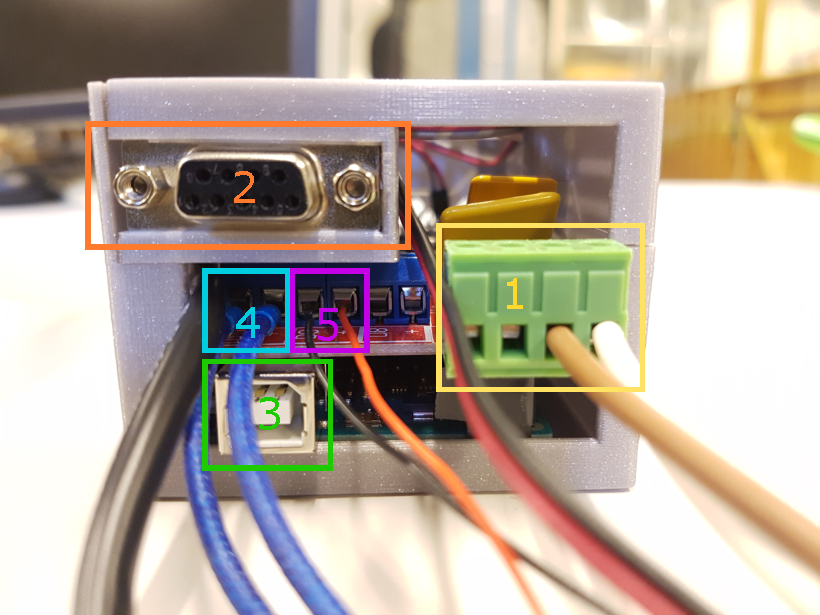
\includegraphics[trim={0.5cm 0 1.5cm 0}, clip, width=\linewidth]{connections_side.pdf}}%
	}%
	\caption{Side of control box}
\end{minipage}\hfill
\begin{minipage}{0.54\textwidth}
	\centering
	{%
	\setlength{\fboxsep}{0pt}%
	\setlength{\fboxrule}{1pt}%
	\fbox{\includegraphics[trim={0.5cm 1.25cm 2cm 0}, clip, width=\linewidth]{connections_top.pdf}}%
	}%
	\caption{Top of control box}
	\label{fig:top_of_control_box}
\end{minipage}
\end{figure}

\begin{enumerate}
\item[1.] 12V power supply connector supplying ramps board with and arduino with power. Brown wire is +12V, white is ground. An internal step-down converter takes +12V and supplies +5V to the arduino board.
\item[2.] Connector port for serial/RS-232 communication. The extruder controller box uses this serial port to receive commands from the computer that is running ROS and to send sensor data to the computer.
\item[3.] USB interface to the arduino. Used for programming the microcontroller. It can also supply the arduino board with +5V, which is enough for it to run and communicate over serial, but it will not power the ramps card (or any of the other devices needing 12V, like the motor, heater or fan). Powering the box/arduino from both the USB (3.) and 12V power supply connector (1.) at the same time is/should be no problem.
\item[4.] Connector for a 12V heater cartridge.
\item[5.] Connector for a 12V heatsink fan. Polarity matter.
\item[6.] Connector for the extruder stepper motor. If connected the wrong way, the motor should move in the opposite and wrong direction.
\item[7.] Connector for thermistor.
\item[8.] Serial (TTL) TX and RX pins. Top pin in figure is D16/TX2 pin on arduino mega, while the second top pin is D17/RX2 pin on arduino.
\item[9.] Power to the RS232 level shifter. Bottom pin in figure is +5V and second bottom pin is ground.
\item[10.] Connections on RS232 level shifter board. From bottom in picture, VCC, GND, TX-O and RX-I. Connect VCC to +5V pin (9.), connect GND to Ground pin (9.), connect TX-O to D17/RX2 pin (8.), and connect RX-I to D16/TX2 pin (8.).
\item[11.] DRV8825, stepper motor driver mounted on top of the ramps 1.4 board.
\end{enumerate}

\newpage
\section{Instructions on use}
\subsection{Hook up the extruder}
Connect a serial cable from the computer to the serial port (2.) on the extruder control box.
Connect a 12V power supply (1.) to the control box. Make sure the power supply can supply 3 Amperes or more to ensure the extruder will operate correctly. A current rating between 0.6 - 3 Amperes can work, but the force produced by the stepper motor and/or the thermal energy produced by the heater cartridge can be lower than what is necessary.

\subsection{Setup}
If you do not already have \href{https://docs.ros.org/en/foxy/Installation}{\texttt{ROS2 foxy}}, \href{https://control.ros.org/getting_started}{\texttt{ros2\_control} and \texttt{ros2\_controllers}}  installed, install them.

Next, create a \href{https://docs.ros.org/en/foxy/Tutorials/Workspace/Creating-A-Workspace.html}{ros2 workspace}, if you have not already done so. 

Navigate to your ros2 workspace and clone the necessary repositories:
\begin{lstlisting}
cd [your_ros2_workspace]/src
git clone https://github.com/mltmyr/am_extruder_tool
git clone https://github.com/mltmyr/am_extruder_simple_ui
git clone https://github.com/mltmyr/am_extruder_msg
\end{lstlisting}

The \texttt{am\_extruder\_tool} package has a git submodule, the RS-232 driver by Teunis van Beelen. We need to fetch that:

\begin{lstlisting}
cd am_extruder_tool
git submodule init
git submodule update
cd ..
\end{lstlisting}

\subsection{Build}

\begin{lstlisting}
source /opt/ros/foxy/setup.bash
cd [your_ros2_workspace]
colcon build
source install/setup.bash
\end{lstlisting}

If building is successful, move on to launching the example in Sec.~\ref{sec:launch_example}. If it fails, you will have to resolve the issue(s) based on the feedback from colcon.

\subsection{Use the ROS2 modules to move and heat filament}\label{sec:launch_example}
Make sure the control box is connected to power and that it is connected to the computer via RS232 cable. Also, ensure that the arduino project \href{https://github.com/mltmyr/extruderCtrl}{\texttt{extruderCtrl}} is loaded and running on the arduino. The stepper motor should make a low buzzing sound and you should not be able to turn the gears because of the motor torque.

To launch the extruder tool demo, run the following command in the terminal:
\begin{lstlisting}
ros2 launch am_extruder_tool_example.launch.py
\end{lstlisting}

Open another terminal and echo the \texttt{joint\_states}. Remember to load/source the ros2 workspace:
\begin{lstlisting}
cd [your_ros2_workspace]
source install/setup.bash
ros2 topic echo /joint_states
\end{lstlisting}
If everything is set up correctly, you should now be able to read the nozzle temperature and filament speed from the data structure being written in the terminal.

To set a reference or target value for the nozzle temperature to $40^\circ \text{C}$, enter the following into a new terminal (remember to source the workspace):
\begin{lstlisting}
ros2 topic pub /filament_heater_controller/commands std_msgs/msg/Float64MultiArray 'data: {40.0}'
\end{lstlisting}
Heating is relatively slow, but after some time, a rise in temperature should be visible on the \texttt{/joint\_states} topic. Set target value to $0.0$ to turn off the heating.

To set a reference or target value for the filament speed to $5\text{mm/s}$, enter the following into a new terminal:
\begin{lstlisting}
ros2 topic pub /filament_mover_controller/commands std_msgs/Float64MultiArray 'data: {5.0}'
\end{lstlisting}
The stepper motor and gears should start to rotate at a speed that will make inserted filament move at $5 \text{mm/s}$. To stop the motor from rotating, set target value to $0.0$. To make the motor rotate the other way, use negative values.

\subsection{Simple RQT plugin}
Setting target values with the help of the \texttt{ros2 topic pub} command is cumbersome and a bit slow. To make it easier to manually control heating and speed of filament a simple RQT plugin was written.

The `Simple extruder gui' RQT plugin can be run from terminal in three different ways:
\begin{enumerate}
\item \colorbox{backcolor}{\texttt{rqt}}. Under plugins, in the top menu, choose \texttt{am\_extruder -> Simple extruder GUI}.
\item \colorbox{backcolor}{\texttt{rqt --standalone am\_extruder\_simple\_ui}}
\item \colorbox{backcolor}{\texttt{ros2 run am\_extruder\_simple\_ui am\_extruder\_simple\_ui}}
\end{enumerate}

Running one of the options, a gui should open. In gui, the current nozzle temperature and filament speed is shown. By entering values in the two fields, the temperature target and speed of the motor can be controlled.

\subsection{Extruder urdf definition}


\begin{figure}[h]
	\centering
	{%
	\setlength{\fboxsep}{0pt}%
	\setlength{\fboxrule}{1pt}%
	\fbox{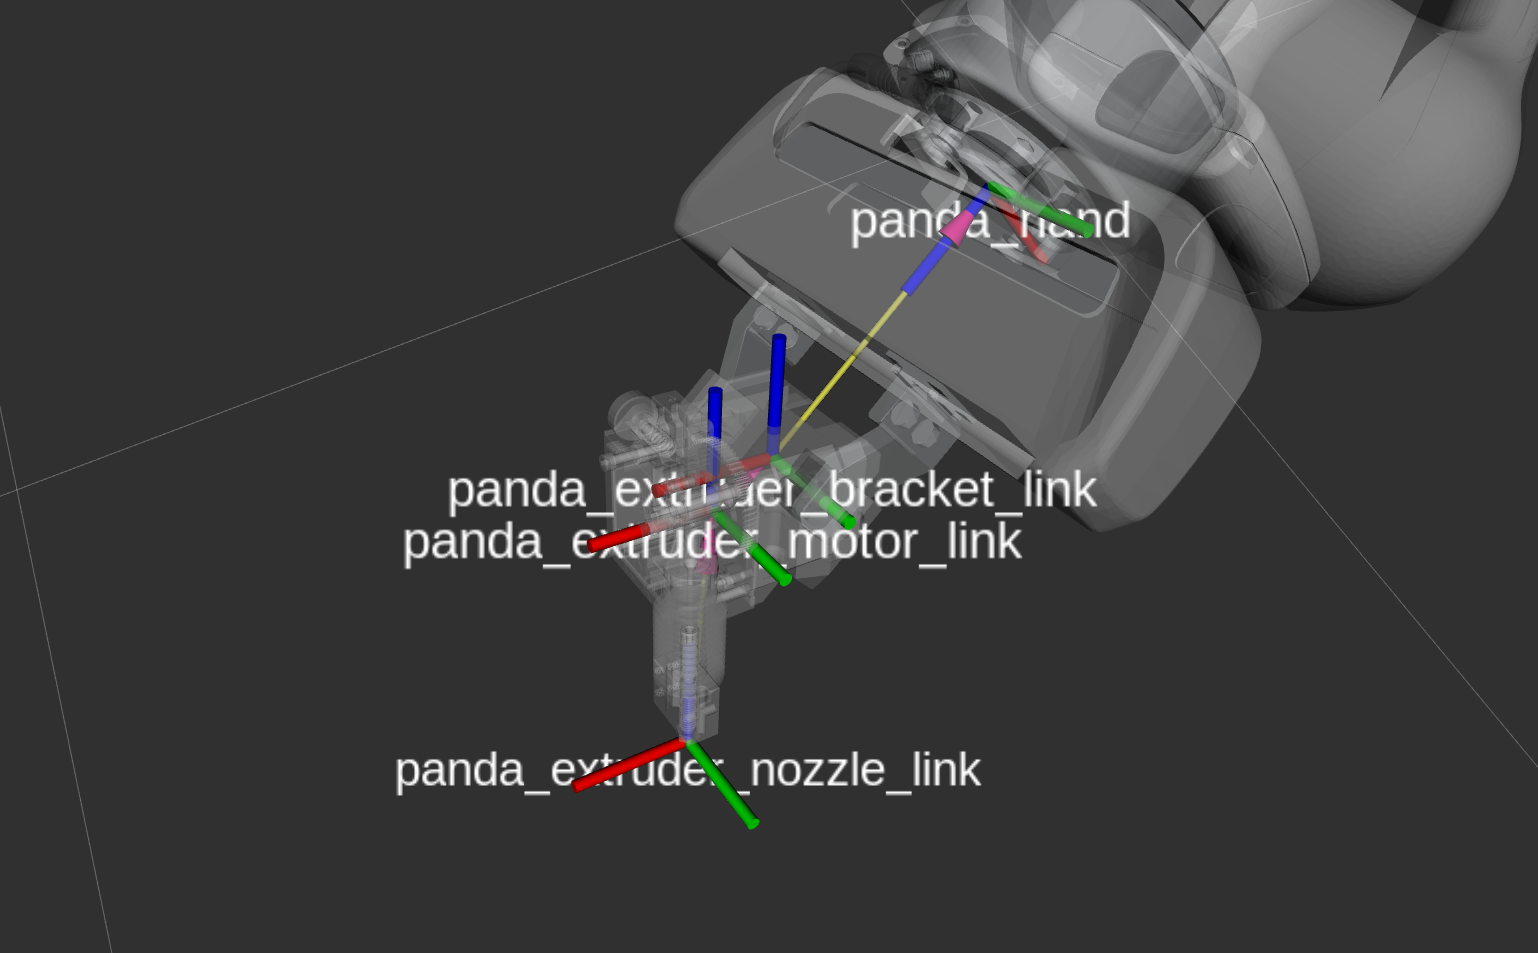
\includegraphics[trim={0 0 0 0}, clip, width=0.85\textwidth]{extruder_coordinate_systems}}
	}%
	\caption{Extruder model and urdf coordinate systems shown with gazebo.}
	\label{fig:extruder_urdf_model_gazebo}
\end{figure}


ROS2\_control and urdf example for integrating into a bigger system,

\newpage
\section{Configure}
\subsection{Configure microstepping level}
Below the stepper motor driver, when it is mounted to the ramps 1.4 board, there are three pairs of pins used for configuring the microstepping level with jumper wires. In the current setup, a microstepping level of 16 microsteps/step is to be used. For the DRV8825, this is configured by adding a jumper wire over the two right most pins, given the orientation of the ramps board in fig. \ref{fig:top_of_control_box}, while leaving the other two pairs of pins unconnected.

If wrong microstepping is used, the motor will either move faster or slower than intended. It will move half as fast with microstepping 32, twice as fast with microstepping 8, four times as fast with microstepping 4, eight times as fast with microstepping 2 and sixteen times as fast with no microstepping.

\subsection{Filament speed and calibration}
The speed at which the filament is moved by the stepper motor when sending a stepping-frequency message to the ramps/arduino board over serial is influenced by several parameters. If, for instance, the filament is to be moved at 1 mm/s, one would have to use these parameters to calculate the stepping-frequency value to be sent over serial. This calculation is done in the ROS2 hardware interface provided in the am\_extruder\_tool package and this calculation needs to be correct in order for the extruder to move the filament at the correct and desired rate.

The low level control of the stepper motor, i.e. voltage and current control of individual windings/phases in the motor, is performed by the DRV8825 stepper motor driver mounted on top of the ramps board. The interface between the stepper motor driver and the arduino board consists of three IO-pins, they are: `enable', `step' and `direction'. The `step'-pin should be pulsed once, each time the motor should move one step in the direction indicated by the `direction'-pin.

To ensure that the `step'-pin is pulsed regularly, and with the correct frequency, a hardware timer is used. A value is entered into the OCRxA register to control the period of the timer. When the timer expires, an interrupt routine is run that toggles the `step'-pin.

\newpage
\section{Software details}

\subsection{Messages over serial}
A simple and lightweight custom message format was created for the communication between the extruder control box and computer running ros.

Each message start with an operation code of one byte and a variable length data field (payload) where the length and format of the payload is implicitly given by the operation code.

There are no acknowledgements and no retransmissions of messages. Therefore, the serial communication is far from robust. But it is sufficient for the current use.

In order for the messages to be as short as possible, nozzle temperature data and stepper motor stepping frequency data is sent over serial as float32 (4 bytes) and not as a string of characters. This makes the data sent over serial unreadable with serial consoles (e.g. PuTTY) that interpret every byte as an ASCII character.

The messages that can be sent between the computer and the extruder control box are explained in Table~\ref{tab:messages_from_computer_to_extruder} and Table~\ref{tab:messages_from_extruder_to_computer}.

\begin{table}[h]
	\centering
	{
	\captionsetup{width=\linewidth}
	\caption{Messages from computer to extruder control box.}
	\label{tab:messages_from_computer_to_extruder}
	}
	\vspace{-0.6em}
	\setlength\tabcolsep{6pt} %default value: 6pt
	\begin{tabular}{>{\centering}p{0.065\linewidth}>{\centering}p{0.08\linewidth}
	p{0.865\linewidth}}
	\toprule
	Opcode & Payload & Purpose \\
	\midrule
	\tabrowA 'H' & float32 & Set nozzle temperature reference in $^\circ\text{C}$ for PID-controller. 5 bytes per message. \\[3pt]
	'X' & float32 & Set stepper motor stepping frequency ($\text{Hz}$). 5 bytes per message. \\[3pt]
	\tabrowA 'B' &  & Blink the debug LED on the arduino/ramps board once. For debugging. 1 byte per message. \\[3pt]
	'Y' &  & Purpose was to start periodic messaging of nozzle temperature and filament speed. This functionality might be disabled in the .ino file. 1 byte per message. \\[3pt]
	\tabrowA 'N' &  & Same as above, but used to turn of periodic messaging. 1 byte per message. \\[3pt]
	'T' &  & Request the controller box to send nozzle temperature in $^\circ\text{C}$ once. Not necessary if nozzle temperature is periodically sent. 1 byte per message. \\[3pt]
	\tabrowA 'E' &  & Request the controller box to send stepper motor stepping frequency ($\text{Hz}$) once. Not necessary if filament feed rate is periodically sent. 1 byte per message. \\[3pt]
	\bottomrule
	\end{tabular}
\end{table}

\begin{table}[h]
	\centering
	{
	\captionsetup{width=\linewidth}
	\caption{Messages from extruder control box to computer.}
	\label{tab:messages_from_extruder_to_computer}
	}
	\vspace{-0.6em}
	\setlength\tabcolsep{6pt} %default value: 6pt
	\begin{tabular}{>{\centering}p{0.065\linewidth}>{\centering}p{0.08\linewidth}
	p{0.865\linewidth}}
	\toprule
	Opcode & payload & Purpose \\
	\midrule
	\tabrowA 'T' & float32 & Message containing nozzle temperature in $^\circ\text{C}$. 5 bytes per message. \\[3pt]
	'E' & float32 & Message containing stepper motor stepping frequency ($\text{Hz}$). 5 bytes per message. \\[3pt]
	\bottomrule
	\end{tabular}
\end{table}


\end{document}